%!TEX root = ../main.tex
\section{System Implementation and Testing}
This section will describe how the system was implemented and tested on both a test setup and the real go-kart setup. 

\subsection{Test Setup}
In order to test subparts of the complete system a test setup was introduced.
It consists of a permanent magnet motor of the type PM5113 with a RMB28MD encoder module mounted with a small distance to the end of the shaft.
The setup furthermore consits of a 74HCT14 level shift interface board and a ?? dual H-bridge and can be seen in figure \ref{fig:small_motor_setup}.
The setup was made and soldered by the supervisors of the project.
The full setup with H-bridge can be used to test the functionality of the Embedded System.
The motor and encoder can be used to test the full system.

\begin{figure}[!h]
	\centering
	\includegraphics[width=0.8\linewidth]{graphics/small_motor_setup}
	\caption[Block diagram of test setup.]{Block diagram of test setup with PM5113 motor.}
	\label{fig:small_motor_setup}
\end{figure}

\todo[inline]{The figure is wrong!! signal should go two times in the level shifter - Mikkel}

\subsection{PWM generating}
To test whether or not the Clarke Park transformation and the PWM generating on the Zybo board was working correctly a test was conducted.
The test setup, described in the previous section, was used.
The three legs of the H-bridge was connected to the control pins for the upper MOSFETS for phase a, b and c.
A constant value for q was chosen and d was set to zero. 
The angle of the rotor was measured and used to do the Clarke Park transformation. 
No current measurements were done, meaning that the only feedback was the angle.
Each of the signals from the output pins of the Zybo board were, in addition to the H-bridge, connected to an electric lowpass filter consisting of a 10 \si{\kilo\ohm} resistor and a 22 \si{\nano\farad} capacitor. 
The voltage across the capacatior was measured by an oscilloscope as the power supply for the H-bridge was turned on.
The measured phase voltages can be seen in figure \ref{fig:small_motor_phases}.
It can be seen that the three phase voltages are created correctly by the Zybo board.
It can also be seen that the rotor is accelerated within a fraction of an electrical revolution, which is expected as there is no torque load. 

\begin{figure}[!h]
	\centering
	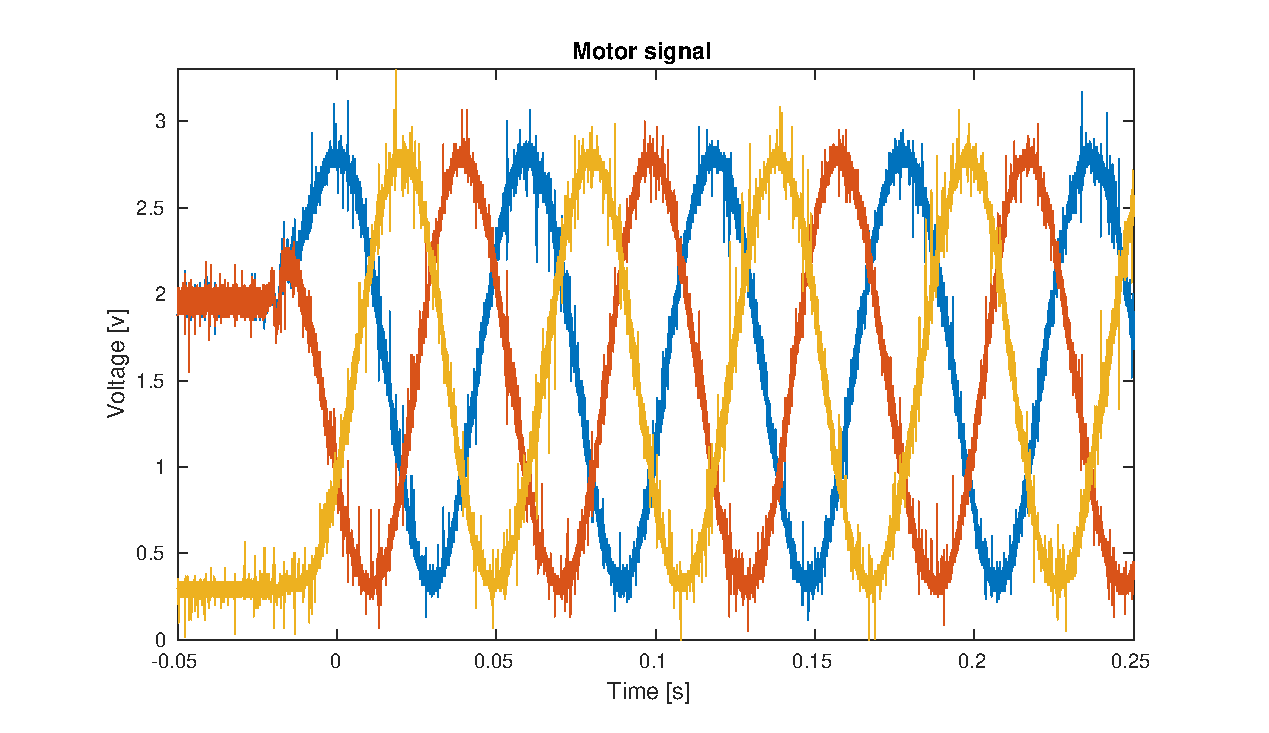
\includegraphics[width=1\linewidth]{graphics/small_motor_phases}
	\caption[Phase voltages.]{Phase voltages measured through a lowpass filter.}
	\label{fig:small_motor_phases}
\end{figure}
